\chapter{Implementierung}

\section{Implementierung des Servers}
\subsection{Parsen der Informationen mit Jsoup}
Um die nötigen Informationen über Foren, Threads und Beiträge für die App
bereitzustellen, müssen diese aus dem bestehenden HTML von readmore.de
ausgelesen werden. Dazu wird das im vorherigen Kapitel schon beschriebene
Framework \Fachbegriff{jsoup} eingesetzt. Um die Informationen auszulesen,
wurden für Foren, Threads und Beiträge jeweils ein eigener Parser implementiert
wie im nachfolgenden UML-Diagramm zu sehen ist.
\begin{figure*}[!htbp]
\centering
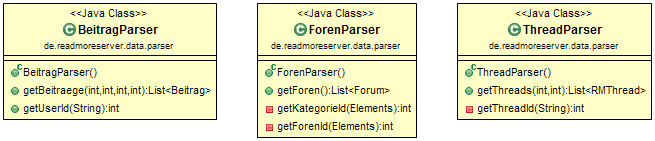
\includegraphics[width=\textwidth]{Bilder/Parser.png}
\caption[Parser für die verschiedenen Forenbereiche]{Parser für die verschiedenen Forenbereiche
 \protect\footnote{eigene Darstellung.} }
\label{dminfo}
\end{figure*}
Jeder der Parser liefert eine Liste vom Typ des jeweiligen geparsten Objekts
zurück, also entweder \Code{Forum}, \Code{RMThread} oder \Code{Beitrag}. Diese
Objekte werden zur internen Datenhaltung verwendet und während des Parsens des
HTML erstellt und mit Daten befüllt. Zusätzlich zu Foren, Threads und Beiträgen,
werden auch die Benutzer in einem eigenen Objekt abgebildet. Dort werden
notwendige Informationen zur späteren Darstellung in der App abgebildet, wie z.B
der Benutzername und der Link zum Avatar des Benutzers. Das Enum \Code{RMStatus}
bildet die Sichtbarkeit des Online Status eines Benutzers ab. Im nachfolgenden
UML-Diagramm wird der Aufbau der einzelnen Objekte dargestellt.
\begin{figure*}[!htbp]
\centering
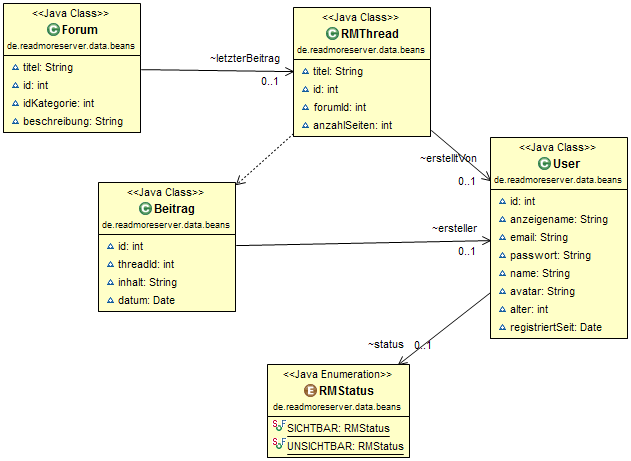
\includegraphics[width=\textwidth]{Bilder/beans.png}
\caption[Objekte für die interne Datenhaltung]{Objekte für die interne Datenhaltung \protect\footnote{eigene Darstellung.} }
\label{dminfo}
\end{figure*}
Das Parsen der HTML-Struktur findet wie schon erwähnt mit \Fachbegriff{jsoup}
statt. Das Framework bietet hierfür viele Möglichkeiten um HTML Elemente anhand
ihrer Klassen, Tags oder anderen Merkmale auszuwählen. Um eine Webseite mit
\Fachbegriff{jsoup} auszulesen, wird über die Methode \Code{connect(URL url)}
das gesamte \Code{Document} mit allen Elementen zurückgegeben. Dieses
\Code{Document} ermöglicht die Selektion der verschiedenen Elemente über die
die bereitgestellten Methoden. Nachfolgend eine Auflistung der wichtigsten
Methoden:
\begin{itemize}
  \item \Code{getElementById(String id)}
  \item \Code{getElementsByAttribute(String key)}
  \item \Code{getElementsByAttributeValue(String key, String value)}
  \item \Code{getElementsByClass(String className)}
  \item \Code{getElementsByTag(String tagName)}
\end{itemize}
Diese Methoden geben je nach Eindeutigkeit der Selektionsparameter ein
\Code{Element} oder die Wrapperklasse \Code{Elements}, die eine Liste
implementiert, zurück. Ein einzelnes \Code{Element} wird nur bei der Methode
\Code{getElementById(String id)} zurückgegeben, da eine Id in HTML Quellcode
stets eindeutig ist. Die Wrapperklasse \Code{Elements} stellt eine Liste von
\Code{Elements} dar, und enthält alle Elemente die den Selektionskriterien
entsprechen. Die implementierten Parser für für Foren, Threads und Beiträge
iterieren über verschiedene \Code{Elements}, um beispielsweise alle Foren der
Forumsstartseite zu erhalten. Diese Iteration ist im nachfolgenden Codebeispiel
zu sehen.
\begin{lstlisting}[caption=Auslesen der Foren im Forenparser, label=forenparser]
public List<Forum> getForen() {
  Document doc = Jsoup.connect("http://www.readmore.de/forums/").get();
  Elements e = doc.getElementsByClass("forum_forums");
  for (Element element : e) {
  Elements foren = element.getElementsByTag("tr");
    for(Element forum : foren) {
      if(forum.children().size() > 4) {
   	    Elements attribute = forum.children();
	    Forum f = new Forum();
	    Elements linkTitel = attribute.get(1).getElementsByTag("a");
	    f.setTitel(linkTitel.text());
	    f.setBeschreibung(attribute.get(1)
	    .getElementsByClass("second_row").text());
	    f.setIdKategorie(getKategorieId(linkTitel));
	    f.setId(getForenId(linkTitel));
	    forenListe.add(f);
      }
    }
  }
}
\end{lstlisting}
In Listing \ref{forenparser} ist auch die Traversierung durch die Baumstruktur
des HTML-Quellcodes zu sehen. Sobald die Informationen aus den einzelnen
Foren-Elementen ausgelesen wurden, wird ein neues \Code{Forum} Objekt erstellt
und mit den ausgelesenen Daten befüllt. Die Parser für Beiträge und Threads
verhalten sich analog.
\subsection{REST Schnittstelle}
Damit die ausgelesenen Daten auch von überall aus abgerufen werden können, wurde
eine REST-Schnittstelle implementiert, die die Daten per HTTP GET im
JSON Format bereitstellt. Um diese zu realisieren, wurde das Framework
\Fachbegriff{Restlet} eingesetzt. Die Klasse \Code{ReadmoreServer} bildet die
Hauptklasse des Servers. Dort wird eine neue Serverkomponente auf Port 8182
gestartet, und das Routing der verschiedenen Anfragen vorgenommen. Es existieren
drei verschiedene Adressen auf die der Server reagiert: \Code{/forum},
\Code{/threads} und \Code{/beitrag}. Eine Anfrage auf \Code{/forum} findet ohne
Parameter statt und gibt ein Json Array mit allen Foren Objekten zurück. Die
Anfragen auf \Code{/threads} und \Code{/beitrag} müssen mit Parametern versehen
werden. Um die Liste mit allen Threads eines bestimmten Forums zu bekommen
müssen die ID des Forums und die ID der Kategorie in der das Forum sich befindet
mitgegeben werden. Die Anfrage um beispielsweise alle Threads im Hardware Forum
von readmore.de abzufragen, würde sich folgendermaßen zusammen setzen:
\Code{/threads?categoryId=91\&forenId=10}.
Um Beiträge einer Seite eines bestimmten Threads zu erhalten müssen außer der
Foren-ID und der Kategorie-ID auch die ID des Threads und die gewünschte Seite
angegeben werden.
\begin{itemize}
  \item Beispiel: 
  \Code{/beitrag?categoryId=91\&forenId=10\&threadId=138573\&seite=1}
\end{itemize}
\begin{figure*}[!htbp]
\centering
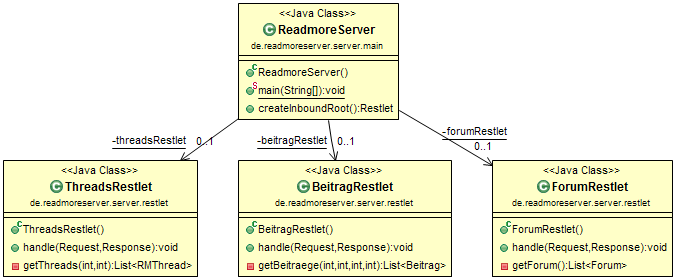
\includegraphics[width=\textwidth]{Bilder/server.png}
\caption[Architektur der REST-Schnittstelle]{Architektur der REST-Schnittstelle \protect\footnote{eigene Darstellung.} }
\label{restuml}
\end{figure*}
Die beschriebenen Anfragen werden in der Hauptklasse des Servers auf
entsprechende \Fachbegriff{Restlets} weitergeleitet, d.h. jede Anfrage 
\Code{/forum}, \Code{/threads} und \Code{/beitrag} wird auf ein eigenes Restlet
weitergeleitet. Dort wird der ankommende GET Request bearbeitet und die
entsprechende Antwort zurückgegeben. Wie im UML Diagramm \ref{restuml} zu sehen,
sind dafür die Restlets \Code{ThreadsRestlet}, \Code{BeitragRestlet} und
\Code{ForumRestlet} zuständig. 
\begin{lstlisting}[caption=Routing der Restlets, label=routing]
public Restlet createInboundRoot() {
  Router router = new Router(getContext());
  router.attach("/threads", threadsRestlet);
  router.attach("/forum", forumRestlet);
  router.attach("/beitrag", beitragRestlet);
  return router;
}
\end{lstlisting}
Wird eine Anfrage an ein Restlet weitergeleitet, wird im Restlet automatisch die
Methode \Code{handle(Request, Response)} aufgerufen. Diese bekommt den Request und eine
Response um eine Antwort zu generieren. Nachfolgend das ForumRestlet als
Beispiel wie die Rückgabe der Forenliste funktioniert.
\begin{lstlisting}[caption=Funktionsweise des ForumRestlet, label=forumrestlet]
public class ForumRestlet extends Restlet {

	@Override
    public void handle(Request request, Response response) {
		List<Forum> forum = getForum();
        String message = null;
        Gson gson = new Gson();
        message = gson.toJson(forum);
        response.setEntity(message, MediaType.TEXT_PLAIN);
    }
    
	private List<Forum> getForum() {
		ForenParser tp = new ForenParser();
		return tp.getForen();
	}
}
\end{lstlisting}
Um eine Liste aller Foren zu erhalten, wird zuerst der \Code{ForenParser}
aufgerufen. Diese Liste wird mithilfe des Frameworks \Fachbegriff{Gson} in ein
JSON Array umgewandelt. \Fachbegriff{Gson} bildet dabei alle Attribute des Java
Objekt in einem Json Objekt ab. Abschließend wird die JSON Nachricht in die HTTP
Response geschrieben. Das JSON Array enthält Forum Objekte im
nachfolgenden Format. 
\begin{lstlisting}[caption=Format der Forum Objekte,label=jsonforum] 
{"titel":"Hardware","id":10,"idKategorie":91,
"beschreibung":"Ecke fuer Technikinteressierte"}
\end{lstlisting}
\section{Implementierung der App}